\documentclass[11pt,a4paper,twoside]{book} % article, report or essay

%\usepackage[margin=3cm]{geometry} %margins



\usepackage[portuges,english]{babel}
\usepackage[utf8x]{inputenc}
\usepackage[T1]{fontenc}
\usepackage{a4wide}
\usepackage{epigraph}
%\usepackage{txfonts}% use Arial && Times New Roman
\usepackage{mathpazo}
\usepackage[pdftex]{color,graphicx}
\usepackage{fancyhdr}
\usepackage{fancyvrb}
%\usepackage{microtype}
\usepackage[printonlyused,withpage]{acronym}
\usepackage{multirow}
\usepackage{cite}
\usepackage{longtable}
\usepackage{moreverb}
\usepackage{verbatim}
\usepackage{listings}
\usepackage{color}

\usepackage{tabularx}

\usepackage{enumerate}
\usepackage{url}
\usepackage{epstopdf}

\usepackage{setspace}

%\linespread{1.3}
\onehalfspace

%\usepackage{amssymb}



\usepackage[pdfauthor={Miguel Goncalves de Araujo PG13367},
			%pdftitle={Asynchronous Replication of Databases in Large Scale},
			pdftitle={Database Replication in Large Scale Systems}
			a4paper,
			pdftex,
			bookmarks,
			colorlinks,
			linkcolor=black,
			urlcolor=black,
			citecolor=black]{hyperref} 
\newcommand{\tab}{\hspace*{2em}}

\usepackage{xspace}

\usepackage{float}
\usepackage{epigraph}

\usepackage{todonotes}

\floatstyle{boxed}
\newfloat{program}{hbt}{lop}
\floatname{program}{Program}


%\lstset{ %
%language=C,                % choose the language of the code
%basicstyle=\small,       % the size of the fonts that are used for the code
%numbers=left,                   % where to put the line-numbers
%numberstyle=\tiny,      % the size of the fonts that are used for the line-numbers
%stepnumber=1,                   % the step between two line-numbers. If it's 1 each line will be numbered
%numbersep=15pt,                  % how far the line-numbers are from the code
%%backgroundcolor=\color{gray},  % choose the background color. You must add \usepackage{color}
%%showspaces=false,               % show spaces adding particular underscores
%showstringspaces=false,         % underline spaces within strings
%%showtabs=false,                 % show tabs within strings adding particular underscores
%%frame=single,	                % adds a frame around the code
%tabsize=2,	                % sets default tabsize to 2 spaces
%%captionpos=b,                   % sets the caption-position to bottom
%breaklines=true,                % sets automatic line breaking
%%breakatwhitespace=false,        % sets if automatic breaks should only happen at whitespace
%%title=\lstname,                 % show the filename of files included with \lstinputlisting; also try caption instead of title
%%escapeinside={\%*}{*)}   % if you want to 
%%add a comment within your code
%morekeywords={refines, refine, @Refines, @Refine, pointcut, call, before, after, around, within, args, target,aspect}            % if you want to add more %keywords to the set
%}

\lstset{%language=Java,
  basicstyle=\small,
  keywordstyle=\color{black}\bfseries\underbar,
  stringstyle=\ttfamily, % typewriter type for strings
  showstringspaces=false,
  columns=fullflexible,
  captionpos=b,
  frame=tb,
  rulesepcolor=\color{black},
  tabsize=2,
  numbers=left,
  firstnumber=1,
  numberfirstline=true,
  numberstyle=\scriptsize,
  mathescape=true
}

\newcommand{\upp}{Uppaal\xspace}
\parindent=16pt
\parskip=4pt

\pdfpagewidth 8.3in
\pdfpageheight 11.7in 


\textwidth 5.9in
\oddsidemargin 0.3in
\evensidemargin 0.02in

%\textwidth 4.8in
%\oddsidemargin 0.35in
%\evensidemargin 1.1in


%\linespread{1.3}
\pagestyle{headings}

\begin{document}



%%%%%% Formal begining of the thesis
\pagenumbering{roman}
	
	\listoftodos
	\newpage
	
	%% cover
	\thispagestyle{empty}
	\thispagestyle{empty}

\setlength{\unitlength}{0.1cm}
\begin{picture}(0,0)

\put(54,-10){
\includegraphics[height=5.5cm]{images/EENG}}

\begin{minipage}[t]{16cm}

~

\vspace{54mm}
\hspace{54mm}
Luís Pedro Zamith de Passos Machado Ferreira\\

\hspace{54mm}
\textbf{Bridging the Gap Between SQL and NoSQL}
\smallskip

%Colocar o subtitulo

\hspace{54mm}

\vspace{55mm}
\hspace{54mm}
Dissertação de Mestrado

\hspace{54mm}
Mestrado em Informática



\hspace{54mm}
Trabalho efectuado sob a orientação de 


\hspace{54mm}
\textbf{Professor Doutor Rui Carlos Oliveira}



\vspace{55mm}
\hspace{54mm}
Outubro 2011

\end{minipage}
\end{picture}
	
	\newpage
	
	\newpage
	\thispagestyle{plain}
	\mbox{}
	%e\setcounter{page}{3}
\noindent{\LARGE\textbf{Declaração}}
\par\vspace{10mm}
\noindent{\textbf{Nome:}} Luís Pedro Zamith de Passos Machado Ferreira
\par\vspace{3mm}
\noindent{\textbf{Endereço Electrónico:}} zamith.28@gmail.com
\par\vspace{3mm}
\noindent{\textbf{Telefone:}} 912927471
\par\vspace{3mm}
\noindent{\textbf{Bilhete de Identidade:}} 13359377
\par\vspace{3mm}
\noindent{\textbf{Título da Dissertação:}} Bridging the Gap Between SQL an NoSQL
\par\vspace{3mm}
\noindent{\textbf{Orientador:}} Doutor Rui Carlos Oliveira
\par\vspace{3mm}
\noindent{\textbf{Ano de conclusão:}} 2011
\par\vspace{3mm}
\noindent{\textbf{Designação do Mestrado:}} Mestrado em Engenharia Informática
\par\vspace{20mm}
\noindent{É AUTORIZADA A REPRODUÇÃO INTEGRAL DESTA DISSERTAÇÃO APENAS PARA
EFEITOS DE INVESTIGAÇÃO, MEDIANTE DECLARAÇÃO ESCRITA DO
INTERESSADO, QUE A TAL SE COMPROMETE.}
\par\vspace{10mm}
\begin{center}
Universidade do Minho, 31 de Outubro de 2011
\par\vspace{3mm}
Luís Zamith Ferreira
\end{center}
%\thispagestyle{empty}
%\newpage
	
	% Epígrafe
	
	\newpage
	\thispagestyle{plain}
	\mbox{}
	
	\newpage
	\thispagestyle{empty}
	\vspace*{0.8\textheight}
\setlength{\epigraphwidth}{7cm}
\renewcommand{\textflush}{flushright}
\epigraph{Future comes by itself, progress does not.}
            {Poul Henningsen}

	\cleardoublepage
	
	%% acknowledgements
	\chapter*{Acknowledgments}
	%\setcounter{page}{5}

\paragraph{}

%Ao apresentar esta dissertação quero agradecer a todos aqueles que, de alguma forma, contribuíram para a sua concretização particularmente:
%\paragraph{}
%- Ao meu orientador, o Professor Doutor José Orlando Pereira pela orientação, acompanhamento e incentivo que me permitiram levar a cabo esta dissertação;
%\paragraph{}
%- Aos meus colegas do Laboratório de Sistemas Distribuídos pela discussão de ideias, entreajuda e apoio "moral";
%\paragraph{}
%- Aos meus pais pelo apoio e suporte fundamental ao longo de todo o meu percurso;

Firstly, I want to thank Prof. Dr. Rui Oliveira for accepting to be my advisor  and for always pushing me to work harder. His support and guidance was of most value to this dissertation.

Secondly, I would like to thank my family for the constant encouragement throughout my studies.

I also thank all the members of the Distributed Systems Group at University of Minho, for the good working environment provided and for always being available whenever I needed help. A special thank to Ricardo Vilaça, for the constant help, and the patience to listen to me all those days. I big thanks to Pedro Gomes, Nelson Gonçalves, Miguel Borges and Francisco Cruz, for the healthy discussions and brainstorms. 

Thanks to all my friends, for their friendship and for their endless support, especially Miguel Regedor, Roberto Machado, Hugo Marinho, André Santos and Pedro Pereira, who helped me grow as an engineer, a student and a person. 

Also thanks to everyone that read this thesis and contributed with corrections and critics.

Although not personally acquainted I would like to thank Jonathan Ellis for the prompt response both by email and on JIRA.  

Last but not the least I thank Carolina Almeida, who's moral support was vital through the duration of this work. 
 
	
	\newpage
	\thispagestyle{plain}
	\mbox{}
	
	
	%% resumo
	\chapter*{Resumo}
	
\paragraph{}


Existe nos dias de hoje uma necessidade crescente da utilização de replicação em bases de dados, sendo que a construção de aplicações de alta performance, disponibilidade e em grande escala dependem desta para manter os dados sincronizados entre servidores e para obter tolerância a faltas.


%A necessidade da utilização de replicação em bases de dados é cada vez maior nos dias de hoje sendo que, a construcção de aplicações de alta performance, disponibilidade e em grande escala dependem desta para manter os dados sincronizados entre servidores e para obter tolerância a faltas.

%There is nowadays an increasing need for database replication, as the construction of high performance, highly available, and large-scale applications depends on it to maintain data synchronized across multiple servers and to achieve fault tolerance.

%A replicação é uma técnica essencial para sistemas de grande escala, alta performance e disponibilidade. A construcção destes sistemas depende da replicação para resolver o problema de manter os dados sincronizados entre servidores e para obter tolerância a faltas.

Uma abordagem particularmente popular, é o sistema código aberto de gestão de bases de dados MySQL e seu mecanismo interno de replicação assíncrona. As limitações impostas pelo MySQL nas topologias de replicação significam que os dados tem que passar por uma série de saltos ou que cada servidor tem de lidar com um grande número de réplicas. Isto é particularmente preocupante quando as actualizações são aceites por várias réplicas e em sistemas de grande escala. Observando as topologias mais comuns e tendo em conta a assincronia referida, surge um problema, o da frescura dos dados. Ou seja, o facto das réplicas não possuírem imediatamente os dados escritos mais recentemente. Este problema vai de encontro ao estado da arte em comunicação em grupo. %tendo em conta as características inerentes a este. Garantias como confiança, ordem, estabilidade, e entrega de mensagens.

Neste contexto, o trabalho apresentado nesta dissertação de Mestrado resulta de uma avaliação dos modelos e mecanismos de comunicação em grupo, assim como as vantagens práticas da replicação baseada nestes. A solução proposta estende a ferramenta MySQL Proxy com plugins aliados ao sistema de comunicação em grupo Spread oferecendo a possibilidade de realizar, de forma transparente, replicação activa e passiva.

Finalmente, para avaliar a solução proposta e implementada utilizamos o modelo de carga de referência definido pelo TPC-C, largamente utilizado para medir o desempenho de bases de dados comerciais. Sob essa especificação, avaliamos assim a nossa proposta em diferentes cenários e configurações.  % As premissas de um melhor desempenho em comparação com o mecanismo de replicação tradicional do MySQL são confirmadas pelos resultados de desempenho.



	
	\newpage
	\thispagestyle{plain}
	\mbox{}
	
	%% abstract
	\chapter*{Abstract}
	
\paragraph{}

There has been a enormous growth in the distributed databases area in the last few years, especially with the NoSQL movement. These databases intend to be almost schema-less and not as strict as their relational counterparts on what concerns the data model, in order to achieve higher scalability. 

Their query API tends to be very reduced and simple (mainly a put, a get and a delete), which grants them very fast writes and reads. All this properties can also be seen as a capability loss in both consistency and query power. There was, therefore, a need to expose the various arguments in favor of and against these properties as well as the attempts that have been and are being made to bring these two technologies closer, and why they are not satisfying enough.

In this context, the work presented in this Master's thesis is the result of evaluating how to take properties from relational and non-relational databases and merge them together. The proposed solution uses Apache Derby DB, Apache Cassandra and Apache Zookeeper having benefits and drawbacks that were pointed out and analyzed.

Finally, to evaluate the proposed and implemented solution we used a workload based on the one defined by the TPC-W benchmark, widely used to benchmark business oriented transactional web servers. Under this specification, we have evaluated our proposal on different scenarios and configurations.
	
	\newpage
	\thispagestyle{plain}
	\mbox{}
		
	
	%% table of contents
	\tableofcontents{}
	
%	\newpage
%	\thispagestyle{plain}
%	\mbox{}
	
	%% list of figures
%	\cleardoublepage
	\listoffigures
    \newpage
    \thispagestyle{plain}
    \mbox{}	
	%% list of tables
%	\cleardoublepage
	\listoftables
	\newpage
	\thispagestyle{plain}
	\mbox{}
    
   \chapter*{List of Acronyms}
    \begin{acronym}[TDMA]
	  \acro{api}[API]{Application Programming Interface}
	  \acro{cql}[CQL]{Cassandra Querying Language}
	  \acro{dbms}[DBMS]{Database Management System}
	  \acro{jdbc}[JDBC]{Java Database Connectivity}
	  \acro{jvm}[JVM]{Java Virtual Machine}
	  \acro{orm}[ORM]{Object Relational Mapper}
	  \acro{ram}[RAM]{Random Access Memory}
	  \acro{rdbms}[RDBMS]{Relational Database Management System}
	  \acro{sql}[SQL]{Structured Query Language}	 
	\end{acronym}
%	\chapter*{}
%	\newpage
\newpage
\thispagestyle{plain}
\mbox{}
\cleardoublepage
	
%%%%%% Content

\pagenumbering{arabic}
	
    %% chapters
	\chapter{Introduction}
        The capability of searching (querying) on a relational system, was first introduced by Edgar Codd's relational model \cite{codd1970relational} in the 1970s. This model is often referred to when talking about the \ac{sql} model, which appeared shortly after and was loosely based on it. The \ac{sql} model~\cite{Chamberlin:1974:SSE:800296.811515} has almost the same structure of the relational model, with the difference that it added a querying language, \ac{sql}, that has since become a \emph{de facto} standard.

In the late 1990's, relational models went from big, monolithic entities to individual users, this made it necessary for them to be more modular and easier to set up. In this context, \acp{rdbms} where at the basis of every dynamic web page available on the Internet. 

Since then, and for most of the web sites today, this way of storing data is still the best and the one with more development and improvement done through the years. However, a new kind of web sites such as social networks (Facebook\footnote{\url{www.facebook.com}}), that are intended to withstand the visit of thousands of clients simultaneously, making it hard to serve all requests with a relational database without a lot of tuning performed by experts. These social networks give much greater importance to the fact the the service is available at all times than to the clients being able to read the last version of such data, since in this use case most of the data is not sensible and different clients can see different sates of that data without compromising the system. This, alongside with an increase in popularity of a new paradigm called cloud computing which is a way to have easy and on-demand increase in computational power with little management and configurational effort, led to the appearance of the \acp{vlsd} which aim to provide the high scalability and availability storing systems these new paradigms needed. 

\acp{vlsd} usually do not use schemas and do not offer complex queries, as joins. They also attempt to be distributed, horizontal scalable, i.e. as machines are added the performance improves, have easy replication support, which means that data will be stored in more than one machine in order to provide availability and partition tolerance. This comes at the cost of providing weak consistency guarantees, because as Eric Brewer's CAP theorem~\cite{Brewer2000} states, it is impossible for a distributed computer system to simultaneously provide \textbf{consistency}, \textbf{availability} and \textbf{partition tolerance}. For a distributed system to be consistent all clients must see current data regardless of updates or deletes, for it to provide availability, all clients will always be able to read and write data, even with node failures and to be partition tolerant, it must continue to work as expected despite network or message loss.

A typical \ac{rdbms} will focus on availability and consistency, having transactional models that provide what is know as ACID properties, which guarantees that the integrity and consistency of the data is maintained despite concurrent accesses and faults. ACID stands for atomicity, consistency, isolation and durability. 

In this context, \textbf{atomicity} means that a jump from the initial state to the result state will occur without any observable intermediate state, giving all or nothing (commit/abort) semantics that is, when a statement is executed, every update within the transaction must succeed in order to be called successful. To be \textbf{consistent} in a relational model scenario means that the transaction is a correct transformation of the state, i.e only consistent data will be written to the database. \textbf{Isolation} is a property that refers to the fact that no transaction should be able to interfere with another transaction, the outside observer sees the transactions as if they execute in some serial order or in other words, if two different transactions attempt to modify the same data at the same time, then one of them will have to wait for the other to complete. The final property is \textbf{durability} which states that once a transaction commits (completes successfully), it will remain so and that the only way to get rid of what a committed transaction has done is to execute an inverse transaction (which is sometimes impossible) thus, a committed transaction will be preserved through power losses, crashes and errors.  

On the other hand, most \acp{vlsd} focus on availability and partition tolerance (Fig. \ref{fig:cap}), relaxing the consistency guarantee, providing eventual consistency~\cite{Vogels2008}. 

\begin{figure}[htb]
  \begin{center}
    \leavevmode
    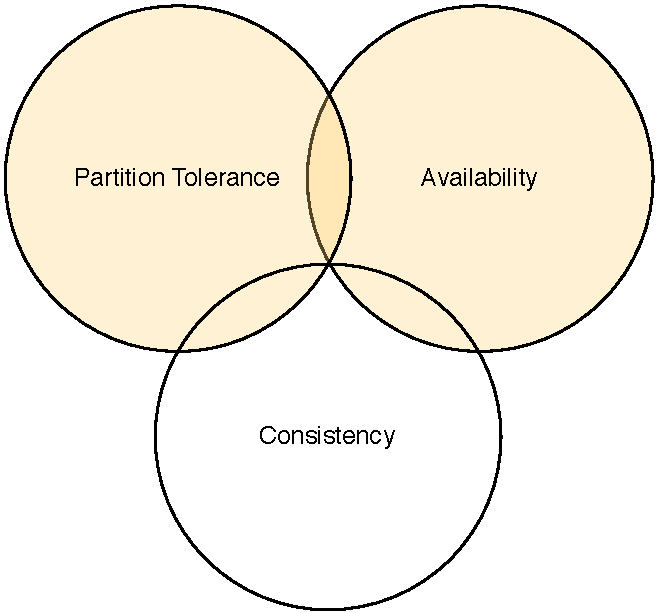
\includegraphics[width=0.5\textwidth]{images/cap}
  \end{center}
  \caption{CAP Theorem}
  \label{fig:cap}
\end{figure}

Eventual consistency means that the storage system guarantees that if no new updates are made to the object, eventually (after the inconsistency window closes) all accesses will return the last updated value. It is seen by many as impracticable for sensitive data, since there is no synchronization that guarantees that updated value will be available at the time of reading. The reality is not so black and white, and the binary opposition between consistent and non consistent is not truly reflected in practice, there are instead degrees of consistency such as strong or causal consistency~\cite{Vogels2008}.

So, on one hand there is the \ac{vlsd} approach, which offers higher scalability, meaning that it can take advantage of having more machines to be able to maintain or even increase its level of performance under bigger loads. On the other hand, a \ac{rdbms} offers more consistency as well as much more powerful query capabilities, leveraging a lot of knowledge and expertise gained over the years \cite{stonebraker2010sql}.  

\section{Problem Statement}

\begin{quote}
If you want to work with a lot of data and be able to run dynamic ad-hoc queries on it, you use a relational database with \ac{sql}. Using a key value store doesn't make any sense for that unless you want to easily be able to distribute your workload on several machines without having to go though the hassle of setting up a relational database cluster. If you want to just keep your objects in a persistent state and have high-performance access to them (e.g. a LOT of web applications), use a key value store.
\end{quote} 
\begin{flushright}in \url{http://buytaert.net/nosql-and-sql}, 25/11/2010\end{flushright}

This separation happens due to the fact that \acp{vlsd} do not provide strong consistency in order to provide partition tolerance and availability, so important in scalable systems. Their reduced \ac{api} makes it simpler and faster to do operations such as a \emph{get} or a \emph{put}. Also, they are prepared from the ground up to replicate data through various machines and even data warehouses.

However, they also have disadvantages as the lack of a standardized query language such as \ac{sql}, making the code vendor specific which in turn makes it less portable. Their simple \ac{api} makes it harder to perform more complex queries and sometimes even impossible since the data is replicated, which makes it hard to maintain an update order and to provide a transactional system with ACID properties. 

These, alongside with the dynamic or non existent schema of these databases, are the main reasons why it is very hard to migrate data and code from a relational database. This kind of migration would save a lot of time and money for companies with huge amounts of code and work done upon relational databases that wish to experience a different type of data storage system.

\section{Objectives}

Migration of data and code is, therefore, something unwanted by developers and managers since it will incur into costs for both, of time and money, respectively. 

According to a blog post by Michael Stonebraker~\cite{stoneEnter}, 61\% of enterprise users are either ignorant about or uninterested in NoSQL\footnote{\acp{vlsd} are subset of NoSQL, since NoSQL does not enforce databases to be distributed}. This happens mainly due to three reasons, because it \textbf{does not provide ACID}, it has a \textbf{low level interface} instead of a high-level language as \ac{sql} and because there is \textbf{no standard} for NoSQL interfaces.

There have been some attempts to make database code the less vendor specific as possible, such as polyglot \acp{orm}\footnote{An orm that outputs different code, according to the database in use, in spite of receiving the same input} as Ruby's DataMapper \cite{DM}, an approach that comes from the fact that even \ac{sql} may differ from \ac{rdbms} to \ac{rdbms} in certain aspects. This portability, however, carries an overhead since it must translate the code to the specific \ac{sql} subset of the required \ac{dbms}.

One problem that \acp{orm} do not solve is migrating legacy \ac{sql} code to a different data model, such as to a \ac{vlsd}. It is exactly this problem that this work aims to tackle, by building a thin layer between the \ac{sql} engine's interpreter and processor, and the actual database underneath it, providing a way to run \ac{sql} queries on top of a \ac{vlsd}.

Alongside with this problem comes another that arise from the limitations of a \ac{vlsd} which is the fact that there is no mechanism to encompass transactions in a \ac{vlsd} and consequently provide the desired ACID properties, which is a problem that this work also addresses and proposes to solve.

To summarize, this work aims:

\begin{itemize}
	\item Allow legacy \ac{sql} code migration to a \ac{vlsd}, taking advantage of a standard language to serve as interface
	\item Provide transactional functionality to the underlying \ac{vlsd}
\end{itemize}

\section{Contributions}

This thesis proposes to provide full \ac{sql} functionality over \ac{vlsd} by altering the \ac{rdbms} underlying storage system.
The major factor in this implementation is that it takes advantage of the scalability and replication features from the \ac{vlsd}, and allies them with the \ac{rdbms} \ac{sql} engine. Also, it provides a completely separate library for transactions in a \ac{vlsd}. 

In detail, we make the following contributions:

\begin{itemize}
	\item \textbf{Prototype database system providing full \ac{sql} functionality over \ac{vlsd}}\\
	   We developed a prototype that allows for \ac{sql} queries to be run over a \ac{vlsd}. In detail, we ported the Apache Derby's query engine to use the Cassandra \ac{vlsd} as its storage layer.
		
	\item \textbf{Distributed transactions library for a \ac{vlsd}}\\
		We developed a library that allows to create and manage transactional contexts enabling to ensure ACID guarantees. 
		
	\item \textbf{Evaluation of the proposed solution}\\
		We evaluate the developed solution using the TPC-W benchmark~\cite{tpcw}, analyzing its behavior under different conditions and configurations comparing its performance to that of a standard \ac{rdbms}. We also evaluated it using the \ac{ycsb} in order to measure the performance of the transactions library without Derby's query engine.
\end{itemize}


\section{Dissertation Outline}

This thesis is organized as follows: Chapter 2 describes the main features of most \acp{vlsd} and some of the implementations; Chapter 3 introduces \ac{sql} and its main functionalities; Chapter 4 describes the modifications made to both Derby and Cassandra in our implementation; Chapter 5 introduces the proposed solution for distributed transactions for \acp{vlsd}; Chapter 6 evaluates the solution implemented using realistic workloads; Chapter 7 describes the related work; and finally Chapter 8 concludes the thesis, summarizing its contributions and describing possible future work. 

		\mbox{}
    \chapter{SQL DBMS and NoSQL}
        

\section{SQL Database Management System}
\label{sec:rdbms}

\begin{quote}
	A method for structuring data in the form of sets of records or tuples so that relations between different entities and attributes can be used for data access and transformation. 
\end{quote} 
\begin{flushright}Burroughs, 1986\end{flushright}
	
This work focuses on the \ac{sql} kind of \ac{dbms} since it is the most widely used and, therefore the one used for the proof of concept.

\subsection{Concept}
A relational database is a database that is perceived by the user as a collection of two-dimensional tables that are manipulated a set at a time, instead of a record at a time.  

It has a rigorous design methodology that is achieved through normalization\footnote{ the process of organizing data to minimize redundancy.}. Moreover it is easily modifiable by adding new tables and rows, even though the schema is rigid, i.e. all the rows in a table must have the same columns. 

One of the main advantages of this approach is the very powerful and flexible join mechanism, based on algebraic set\footnote{ group of common elements where each member has some unique aspect or attribute} theory, providing fast responses to complex queries.

Since its appearance a lot of work has been done in order to fasten the processing, from multi-threaded or parallel servers to the usage of indexes\footnote{ used to find rows with specific column values fast at the cost of slower writes and increased storage space.} and fast networks. 

\subsection{Components}
Every \ac{dbms}  has four common components, its building blocks. They may vary from one system to another, but the general purpose of each of these components is always the same.

\subsubsection{Modeling language}
First of all, there is the modeling language, that defines the schema of the database, that is, the way it is structured. These models range from the hierarchical, to the network, object, multidimensional and to the relational, that can be combined to provide an optimal system. The most commonly used is the relational structure, that uses two-dimensional rows and columns to store data, forming records, that can be connected to each other by key values. 

In order to get more practical and faster systems, the most used model today is actual a relational model embedded with \ac{sql} .

\subsubsection{Data Structure}
Every database has its own data structures (fields, records, files and objects) optimized to deal with very large amounts of data stored on a permanent data storage device (which is obviously slow, when compared to volatile memory).

\subsubsection{Database Query Language}
A database query language allows users to interrogate the database, analyze and update data, and control its security. Users can be granted different types of privileges, and the identity of said users is guaranteed using a password. The most widely used language nowadays is \ac{sql} , which provides the user with four main operations, know as CRUD (Create, Read, Update, Delete).  

\subsubsection{Transactions}
A \ac{rdbms} should have a transactional mechanism that assures the ACID properties:
\begin{description}
	\item[Atomicity] A jump from the initial state to the result state without any \textbf{observable} intermediate state. All or nothing (Commit/Abort) semantics that is, when a statement is executed, every update within the transaction must succeed in order to be called successful.
	\item[Consistency] The transaction is a correct transformation of the state, i.e only consistent data will be written to the database.
	\item[Isolation] No transaction should be able to interfere with another transaction. The outside observer sees the transactions as if they execute in some serial order. That is, if two different transactions attempt to modify the same data at the same time, then one of them will have to wait for the other to complete.
	\item[Durability] Once a transaction commits (completes successfully), it will remain so. The only way to get rid of what a committed transaction has done is to execute an inverse transaction (which is sometimes impossible). A committed transaction will be preserved through power losses, crashes and errors. 
\end{description}

Which guarantees that the integrity and consistency of the data is maintained despite concurrent accesses and faults.  

\section{NoSQL}
\label{sec:nosql}
NoSQL \cite{seeger09} is a term used to refer to database management systems that, in some way, are different from the classic relational model. These systems, usually, do not use schemas and avoid complex queries, as joins. They also attempt to be distributed, open-source, horizontal scalable (see chapter \ref{chap:cass}), eventually consistent \cite{Vogels2008}, have easy replication\footnote{``Replication is the process of sharing information between databases (or any other type of server) to ensure that the content is consistent between systems.'' - \url{http://databases.about.com/cs/administration/g/replication.htm} (10/1/2011)} support and a simple \ac{api}.

The term was first used in 1998 as the name of a relational database that did not provide a \ac{sql} interface. It resurfaced in 2009, as an attempt to label a set of distributed, non-relational data stores that did not, necessarily, provide ACID guarantees.

The ``no:sql(east)'' conference in 2009, was really what jump started the current buzz on NoSQL. A wrong way to look at this movement is as an opponent to the relational systems, as the its main goals are to emphasize the advantages of Key-Value Stores, Document Databases, and Graph Databases.

\subsection{Architecture}
Relational databases are not tuned for certain data intensive applications, as serving pages on high traffic websites or streaming media, therefore show poor performance in these cases. Usually they are tuned either for small but frequent read/write transactions or for large batch transactions, used mostly for reading purposes. On the other hand, NoSQL addresses services that have heavy read/write workloads, as the Facebook's inbox search \cite{lakshmanMalik}.

As stated earlier, NoSQL often provides weak consistency guarantees, as eventual consistency \cite{Vogels2008}, and many of these systems employ a distributed architecture, storing the data in a replicated manner, often using a distributed hash table \cite{Tanner}. This allows for the system to scale out with the addition of new nodes and to tolerate failure of a server.

\subsection{Taxonomy}
NoSQL implementations can be categorized according to the way they are implemented, being that they are a document store, a key/value store on disk or a cache in \ac{ram}, a tuple store, an object database, or as the one used in this work, an eventually-consistent key/value store.\\

The differences between NoSQL and \ac{rdbms} will be summarized in Table \ref{tab:diff}:\\

\begin{table}[h!b!p!]
\scalebox{0.92}{
\begin{tabular}{|*{7}{c|}}
	\hline
	 &Schema&Consistency&Queries&Usage&Storage\\
	\hline
	\multirow{2}{*}{NoSQL}&Usually&\multirow{2}{*}{Eventual}&\multirow{2}{*}{Simple}&Read/Write&\multirow{2}{*}{Replicated}\\
	     &none   &        &      &Intensive&\\
	\hline
	\multirow{3}{*}{RDBMS}&\multirow{3}{*}{Yes}&\multirow{3}{*}{ACID}&\multirow{3}{*}{Complex}&Small frequent&\multirow{3}{*}{Local}\\
	                      &   &    &       &read/write or&\\
		                  &   &    &       &long batch transactions&\\
	\hline	
\end{tabular}
}
\caption{Differences between NoSQL and RDBMS}
\label{tab:diff}
\end{table}	  

\section{Case Study}
To accomplish the goals proposed in the introduction, there was a need to choose one \ac{rdbms} and one NoSQL implementation in order to develop a solution as both a proof of concept and a way to get real results. The chosen systems were the Apache Derby as the database manager and the Apache Cassandra as the NoSQL implementation for the following reasons:

\begin{itemize}
	\item Written in Java
	\item Open-source
	\item Previous experience with both
\end{itemize}

		

   	    \mbox{}	
	\chapter{Related Work}
	    Our work spans over several areas such as altering the processor part of an \ac{sql} query engine and distributed transactions. There is also some work on high level interfaces for \acp{vlsd} that we find is worth mentioning.

\section{SQL over Memory}
The idea of patching Derby so that the data is stored in a different way than normal is not entirely new and was firstly introduced by Knut Magne Solem~\cite{derbyPatch}. In his approach all the tables whose name began with \emph{MEM} were stored in memory, as opposed to our approach which stores in Cassandra all the tables whose name starts with \emph{TUPLE}.

\section{Distributed Transactions}

Transactions become difficult under heavy load. When you first attempt to horizontally scale a relational database, making it distributed, you must now account for distributed transactions, where the transaction isn’t simply operating inside a single table or a single database, but is spread across multiple systems. In order to continue to honor the ACID properties of transactions, you need a transaction manager to orchestrate across the multiple nodes.

There are many leader election algorithms but they all have the same input and output. At the beginning there is a set of nodes in a network, unaware of which of them is the leader, after the protocol they all recognize a particular, unique node as the leader.

Assuming that the leader is already elected, a simple way to complete a distributed transaction in an atomic manner is for the coordinator to communicate the commit or abort request to all of the participants in the transaction and keep repeating the request until all of them have acknowledged that they have carried it out. This is called one-phase commit protocol~\cite{coulouris2005distributed} and is inadequate because it does not allow a server to make a unilateral decision to abort a transaction. 

\subsubsection{Two-phase commit protocol}

The two-phase commit protocol is designed to allow any participant to abort its part of a transaction which, by the atomicity requirement, means the whole transaction must be aborted. 

In the first phase of the protocol the coordinator asks all of the participants if they are prepared to commit and in the second it tells them to commit/abort the transaction. Once a participant has voted to commit a transaction it is not allowed to abort it, therefore a participant must before make sure it will be able to carry out its part of the protocol, before committing to it. 

\begin{table}[h!]
\centering
  \begin{tabular}{  l  p{8cm}}
	\toprule
	Operation & Description\\
    \midrule
    \emph{canCommit?(trans) $\rightarrow$ Yes/No} & Coordinator asks if it can commit a transaction. Participant replies with vote.\\  
    \emph{doCommit(trans)} & Coordinator tells participant to commit its part.\\
    \emph{doAbort(trans)} & Coordinator tells participant to abort its part.\\
    \emph{haveCommited(trans,participant)} & Participant tells the coordinator it has commited.\\
    \emph{getDecision(trans) $\rightarrow$ Yes/No} & Participant asks for decision after it has voted. Used to recover from server crashes or delayed messages.\\
	\bottomrule
  \end{tabular}

\caption{Operations for two-phase commit protocol (based on \cite{coulouris2005distributed})}
\label{tab:2pc_ops}
\end{table}

Using the operations defined in table \ref{tab:2pc_ops}, a successful run of the protocol with one coordinator and one participant is as shown by figure \ref{fig:2pc_run}.

\begin{figure}[htb]
  \begin{center}
    \leavevmode
    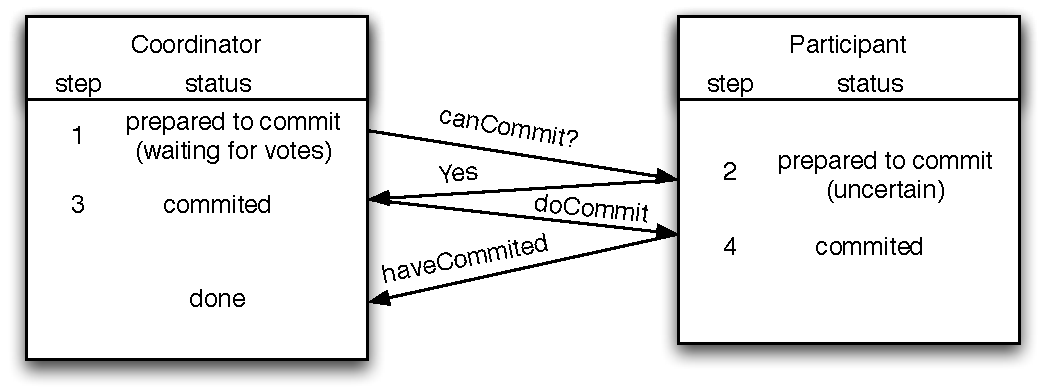
\includegraphics[width=0.9\textwidth]{images/2pc}
  \end{center}
  \caption{Two-phase commit successful run\cite{coulouris2005distributed}}
  \label{fig:2pc_run}
\end{figure}

\subsection{CloudTPS}
One particular implementation of distributed transactions, i.e. offers transactional guarantees (ACID) over a \ac{vlsd}, is CloudTPS~\cite{cloudTPS} which chooses to provide strong consistency at the cost of the possibility of becoming unavailable when facing network partition. In order to provide full transactional guarantees it introduces the concept of \acp{ltm} which are various parts of a transaction manager called transaction processing system, each of them is responsible for a part of the data and for processing certain parts of the transaction.

Since a transactional system must maintain the ACID properties even in the case of server failures, the data items and transactions state are replicated to multiple \acp{ltm} and consistent data snapshots are periodically checkpointed to the cloud storage system in order to guarantee the durability of each transaction.

The client can submit a transaction to any \ac{ltm} that is responsible for one of the accessed item, which then acts as the coordinator of the transaction across all \acp{ltm} responsible for the data items needed by the transaction, which is implemented using the two-phase commit protocol where the other \acp{ltm} are the participants.


\section{High Level Interfaces for a \ac{vlsd}}
\acp{vlsd}' query interfaces are in general very low level and do not conform to any type of standard which, as has been pointed out, leads to many problems including portability of code. There have been several projects that have proposed different high level interfaces for the \acp{vlsd} in order to mitigate this problem. 

\subsection{Object Mapper}

Using object mapping tools in order to allow to bypass the lower level interfaces of Cassandra is one the possible approaches, and is the one taken by the Cassandra Object Mapper~\cite{Pi}. 

In this project the user has at its disposal generic object interfaces like JPA and JDO that allow him to use the underlying database in an almost transparent way, which greatly simplifies the reading and writing of data. This transparency also brings the advantage of aiding in the migration of existent solutions and allowing the mix of different types of data stores under the same code base.  

The underlying store can be a Cassandra cluster which will, therefore, be available to the user through one of those interfaces with all their expressiveness and features, such as JDO class annotations.

One of the downsides of this solution is that it offer no transactional guarantees and therefore some of features that would be expected in this kind of the tool are thereby unavailable to the user. 

\subsection{Hive}
Hive~\cite{Thusoo:2009:HWS:1687553.1687609} was initially developed at Facebook and is now an Apache project. It is built on top of Apache Hadoop and facilitates querying and managing of large datasets in distributed storage by providing a mechanism to impose structure on a variety of data formats and access to files stored directly in Apache HDFS or in other storage systems. 

It defines a simple SQL-like query language, called \emph{HiveQL}, whose queries are executed via MapReduce with the particularity that there is no specific data format, it works on Thrift and allows for the creation of specialized data formats. Also, it enables users to plug in custom map-reduce scripts into queries.

Hive is not designed for online transaction processing and it is best used for batch jobs over large sets of append-only data since what it values most is scalability, extensibility, fault-tolerance and a loose coupling between it and its input formats. 

\subsection{\acl{cql}}

The \ac{cql} \cite{cql}, is a really novel approach to this matter, being developed by Eric Evans. His idea, is to develop a \ac{sql} like query language on top of Cassandra, bypassing an \ac{sql} interpreter altogether at the expense of not being compatible with actual \ac{sql}  code. Still, this would allow for much faster adaptation to Cassandra, for people with relational background. 

\ac{cql} has been released with Cassandra new stable version (0.8), and a select query will look somewhat like this \cite{cqlSelect}:

\begin{center}
\begin{verbatim}
    SELECT (FROM)? <CF> [USING CONSISTENCY.<LVL>] WHERE 
       <EXPRESSION> [ROWLIMIT X] [COLLIMIT Y] [ASC|DESC]
\end{verbatim}
\end{center}

And would be replacing a lot of old methods for retrieving data as \emph{get()}, \emph{get\_slice()}, \emph{get\_range\_slices()}, and so on.	

At the time of writing there are still some features to be implemented~\cite{cqlbbw}, such as \emph{ALTER} and prepared statements and some SQL features that will not be implemented at all, as joins and update\footnote{Since cassandra 0.7 the updates are viewed as a special case of insert}.

		\mbox{}	
    \chapter{Derby}
       Apache Derby is an open-source Java \ac{rdbms}, that has a very small footprint (about 2.6MB of disk-space for the base engine and embedded \ac{jdbc} driver \cite{derbySite}). The on-disk database format used in Derby is portable and platform-independent, meaning that the database can be moved from machine to machine with no need to modify the data, and that the database will work with any derby configuration \cite{derby10}. 

A Derby database exists within a system (Fig. \ref{fig:derbystruct}), composed by a single instance of the Derby database engine and the environment in which it runs. It consists of zero or more databases, a system-wide configuration and an error log, both contained in the system directory \cite{derbyDev10}.

\begin{figure}[htb]
  \begin{center}
    \leavevmode
    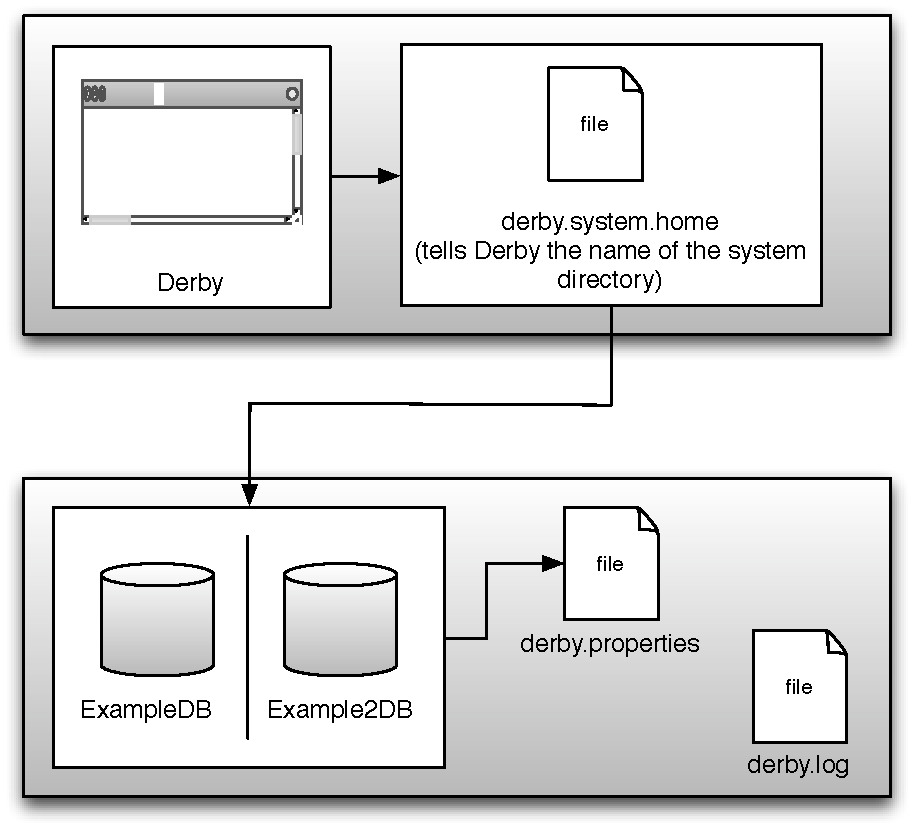
\includegraphics[width=0.5\textwidth]{images/derbystruct}
  \end{center}
  \caption{Derby System Structure}
  \label{fig:derbystruct}
\end{figure}

\section{Data Model}
Derby's data model is relational, implying that data can be accessed and modified using \ac{jdbc} and standard \ac{sql}. The system has, however, two very different basic deployment options (or frameworks), the simple embedded option and the Derby Network Server option \cite{derby10}. 

\begin{description}
	\item[Embedded] In this mode Derby is started by a single-user Java application, and runs in the same Java virtual machine (JVM). This makes Derby almost invisible to the user, since it is started and stopped by the application, requiring very little or no administration. This has the particularity that only a single application can access the database at any one time, and no network access occurs. 
	\item[Server (or Server-based)] In this mode Derby is started by an application that provides multi-user connectivity to Derby databases across a network. The system runs in the JVM that hosts the server, and other JVM's connect to it to access the database.
\end{description}	

\section{Querying}
Querying in Derby is done, as previously mentioned, with the usage of \ac{sql}, more precisely features from \ac{sql}-92 \cite{derbySQL}.

\ac{sql} scope includes data insert, query, update and delete, schema creation and modification, and data access control, and is the most widely used language for relational databases \cite{SQLintro}. \ac{sql} statements are executed by a database manager, who also has the function transforming the specification of a result table into a sequence of internal operations that optimize data retrieval. This transformation occurs in two phases: preparation and binding.

All executable \ac{sql} statements must be prepared before they can be executed, with the result of this preparation being the executable or operational form of the statement. The method of preparing an \ac{sql} statement and the persistence of its operational form distinguish static \ac{sql} from dynamic \ac{sql} \cite{SQLibm}.

\section{Consistency}
Derby databases provide ACID guarantees, according to the ACID test \cite{derbydevIBM}. This means that operations with the database can be grouped together and treated as a single unit (atomicity), it makes sure that either all the operations in this single unit (\emph{transaction}) are performed, or none is (consistency), also, independent sets of database transactions are performed so that they don't conflict with each other (isolation) and it also guarantees that the database is safe against unexpected terminations (durability).

\section{Patching Derby}

The idea of patching Derby so that the data is stored in a different way is not entirely new and was firstly introduced by Knut Magne Solem\cite{derbyPatch}. In his approach all the tables whose name began with \emph{MEM} were stored in memory, following the same strategy, our approach stores in Cassandra all the tables whose name starts with \emph{TUPLE}.

This implies re-writing all the classes and methods from the access part of the Derby engine, that uses a BTree by default and therefore are in the namesake package. As this implementation uses a Tuple Store, the name of the package was also tuplestore.

When rewriting this classes some optimizations were made, such as the reutilization of connections since Derby creates one physical connection to the underlying database for each transaction, which could mean a reasonable overhead when a new one was created due to the cost of establishing the connection. To circumvent this, a pool of connections is created and if there is one free it is used, otherwise a new connection is opened, preventing some of the overhead. 

\subsection{Records}

\subsection{Indexing}
Indexing is a way of sorting a number of records on multiple fields. Creating an index on a field in a table creates another data structure with the field value, and a pointer to the primary record. 

The downside to indexing is that these indexes require additional space on the disk and processing time when inserting new data.

\subsubsection{Derby Indexes}
Parallel to the actual record handling classes, there are the ones responsible for the indexes, which can be of one of three types:

\begin{description}
	\item[Primary] Refers to primary keys. There can only be one per table and it must unambiguously match one, and only one, record.
	\item[Unique] Resemble ordinary (secondary) indexes, except they prevent duplicates from being added.
	\item[Secondary] Secondary or Ordinary indexes serve the same purposes as primary indexes, but on different values than the primary key.
\end{description} 

The creation of an index in the patched version of Derby depends on its type. 

In the case where it is a primary index, Derby is informed about it (through a flag), but no actual index is created, since the record already contains that information and is indexed for it.

On the rest of the cases, an index is created according to the model defined in chapter \todo{capitulo do modelo de dados do cassandra}.

When fetching information that is indexed, Derby first estimates the cost of fetching using the index or not, based on the number and size of the rows, and acts accordingly.

\begin{figure}[h]
  \centering    
  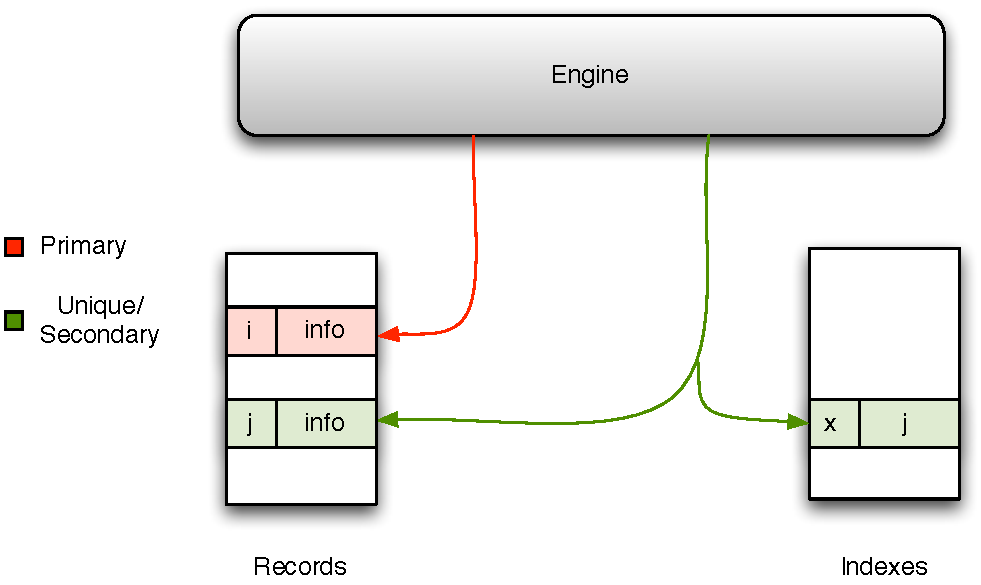
\includegraphics[width=0.9\textwidth]{images/derbyindexes}
  \caption{Derby Indexes}
  \label{fig:derbyindexes}
\end{figure}


\subsection{Scans}

\todo[inline]{Explicar como é feito uma range query no Derby}  

When performing a scan that involves fetching a row through an index, Derby gets the row for that index from which it extracts the location of the actual record and then does a second fetch, this time to the location pointed by the index.

This is fine for unique and secondary indexes, but as explained in the previous section, in the case of primary indexes there is no need for the creation of a specific row for the index, thus making this two fetches mechanism redundant. Since this redundancy meant an unnecessary access to the database, which could incur in a large overhead, this matter had to be addressed. 

The way this was solved was by storing in memory the whole row fetched in first place (through the index) and passing it on alongside with the actual record location. This allows for the controller of the fetch to use the information in memory, when it is available.   









   	   \mbox{}
	\chapter{Cassandra}
	\label{chap:cass}
       Cassandra \cite{will10} was created by Facebook and is based on Dynamo \cite{Hastorun2007} and BigTable \cite{Chang2008}. The main goals of this system have been, from scratch, to be highly scalable, decentralized and fault tolerant.

Eric Brewer's CAP theorem \cite{Brewer2000} states that it is impossible for a distributed computer system to simultaneously provide all three of the following guarantees:
\begin{itemize}
	\item Consistency
	\item Availability
	\item Partition Tolerance
\end{itemize}

The NoSQL implementations, including Cassandra, focus on the last two, relaxing the consistency guarantee, providing eventual consistency. Usually, NoSQL members are key-value stores, that have nearly no structure in their data model, apart from what can be seen as an associative array. On the other hand, Cassandra is a column oriented database system, with a rather complex data model, that is described below.

Cassandra is built to optimize reads, therefore it does no processing when fetching the stored data. All the processing, as sorting, indexing (column families can be used to create indexes), and so on, is done when storing the said data, which is basically the opposite of what happens on the classical models (\ac{rdbms}).

\section{Data Model}
In this section the data model of Cassandra \cite{sarkissian09} will be explained from the most basic component to the most complex, with some detail, since this is very different from the relational data model most people are used to, and takes some time to digest and understand.

The basic building block of Cassandra are columns (Fig. \ref{fig:column}), that consist of a tuple with three elements, a name, a value and a timestamp.

\begin{figure}[htb]
  \begin{center}
    \leavevmode
    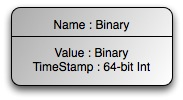
\includegraphics[width=0.3\textwidth]{images/column.jpg}
  \end{center}
  \caption{Cassandra Column}
  \label{fig:column}
\end{figure}

In the next level of complexity there is the SuperColumn (Fig. \ref{fig:supercolumn}), that is also a tuple, but only has two elements, the name and the value with the particularity that the value is a map of keys to columns (this key has to be the same as the column's name).

\begin{figure}[htb]
  \begin{center}
    \leavevmode
    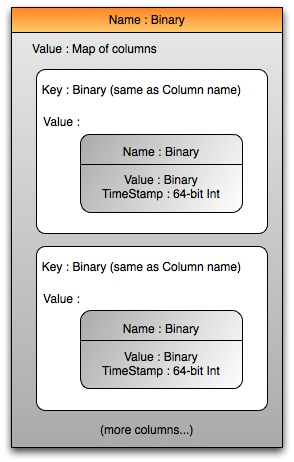
\includegraphics[width=0.4\textwidth]{images/supercolumn.jpg}
  \end{center}
  \caption{Cassandra SuperColumn}
  \label{fig:supercolumn}
\end{figure}

The maximum level of complexity is achieved with the Column Families, which ``glue'' this whole system together, it is a structure that can keep an infinite number of rows (super columns), and has a name, and a map of keys to rows as shown in picture \ref{fig:columnfamily}. Every operation under a single row key is atomic per replica, despite the number of columns affected.

Applications can specify the sort order of columns within a column family, that can be based on the name or on the timestamp. The system allows for multiple keyspaces (tables), but almost all deployments have only one in their schema.

\begin{figure}[!htb]
  \begin{center}
    \leavevmode
    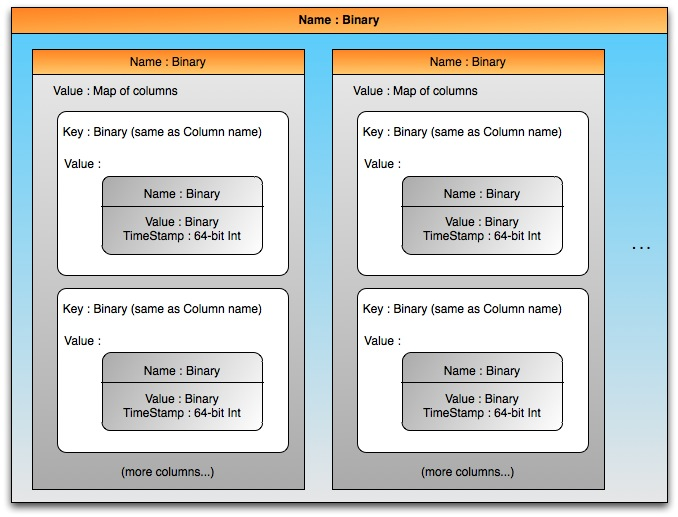
\includegraphics[width=0.8\textwidth]{images/columnfamily.jpg}
  \end{center}
  \caption{Cassandra ColumnFamily}
  \label{fig:columnfamily}
\end{figure}

There is a variation of ColumnFamilies that are SuperColumnFamilies. The only difference is that where a ColumnFamily has SuperColumns with maps of columns, a SuperColumnFamily has SuperColumns with maps of SuperColumns. 

\section{Querying}
Cassandra's \ac{api} is what defines it's querying capabilities, and consists of three simple methods \cite{lakshmanMalik}:

\begin{itemize}
	\item \emph{insert(table, key, rowMutation)}
	\item \emph{get(table, key, columnName)}
	\item \emph{delete(table, key, columnName)}
\end{itemize}	

In the method signatures above, \emph{columnName} can refer to a specific column in a column family, a column family, simple or super, or a column in a supercolumn. The \emph{rowMutation} specifies the changes to the row in case it was already there, or the row to be added.

\section{Consistency}
Cassandra allows clients to specify the desired consistency level on reads and writes, based on the replication factor previously defined in a configuration file, present in every cluster. Notice that if R + W > Replication Factor, where R is the number of nodes to block for on read, and W the ones to block for on write, the most consistent behavior will be achieved\footnote{Because the repair replication process only requires a write to reach a single node to propagate, a write which ``fails'' to meet consistency requirements will still appear eventually as long as it was written to at least one node.}.\\

Cassandra uses replication to achieve high availability and durability. Each data item is replicated at N nodes, where N is the afore mentioned replication factor, assigning each key to a coordinator node (chosen through consistent hashing\footnote{``Consistent hashing is a scheme that provides hash table functionality in a way that the addition or removal of one slot does not significantly change the mapping of keys to slots. By using consistent hashing, only K/n keys need to be remapped on average, where K is the number of keys, and n is the number of slots.'' in Wikipedia, 13/12/2010}), that in addition to storing locally each key within his range, replicates these keys at the N-1 nodes in the consistent hashing ring. 

Cassandra system elects a leader amongst its nodes using Zookeeper \cite{Junqueira2007}, that is contacted by all joining nodes, and tells them for what ranges they are responsible. The leader also makes an effort for maintaining the invariant that no node is responsible for more than N-1 ranges in the ring. 

In Cassandra every node is aware of every other node in the system and, therefore the range they are responsible for.

       \mbox{}
	\chapter{Fully Distributed Transactional Model}
	\label{chap:fdtm}
       With these changes to Derby we have gained scalability, fault and partition tolerance and kept durability. This of course came with the cost of loosing atomicity\footnote{Cassandra provides atomicity at the row level, which is fine when doing separate inserts at a time, but is not good enough when performing batch inserts, in our model}, isolation and consistency (we have eventual consistency). 

In practical terms this means that transactions are not be possible with this system. To overcome these limitations we built a distributed transaction system that takes advantage of Cassandra's peer to peer architecture with the exception of a Zookeeper cluster to manage the locks. This cluster and why it is not a big limitation to the overall performance of the system are further explained in section \todo{secção do Zk e Cages}.

\section{Algorithm}
The adopted algorithm (Fig. \todo{algoritmo}) combines a mechanism of locks and a write ahead log with Cassandra's provided atomicity and idempotent operations.

\missingfigure{O algoritmo transaccional}

\section{Locks}
Before the actual transaction can start, it must acquire the locks for the rows (or entire tables) it is going to use. These locks are kept in a Zookeeper cluster, using a library called Cages.

The actual lock mechanism works by first asking for a lock for the table called \emph{any\_or\_all}, when attempting to lock the entire table this is a write lock, otherwise it is a read lock. In the second case there is a second step of asking for locks on the rows we need, since there can be many threads with read locks on the same table at the same time. This means that all threads can pass on to ask for locks in the rows, unless there is another wanting to lock the whole table. 

Each lock is represented by a Path class, that encapsulates the path to lock as well as its type (table lock or not) and provides the necessary primitives to work with it. 

Still this mechanism is not enough because it does not prevent deadlocks\footnote{If two threads want locks A and B, and one of them gets A and the other B, they will both be waiting on the other, which is the definition of a deadlock}. In order to do this, there has to be a globally accorded way of ordering the paths of the locks, for this we first compare the nesting of the path (table locks are less nested and therefore are sorted first), then we compare the actual name of the table\footnote{using Java strings default compareTo method} and at last, in the case of rows of the same table, we compare the name of the row. This comparison in done with a Comparator class, which provides a way to change the way paths are compared without changing the code of the actual system.

\subsection{Cages}
\todo[inline]{Falar do cages e como funciona}

\subsection{Zookeeper}
\todo[inline]{Falar um bocadinho de zookeeper, com principal enfase nos observers}



      
   	   \mbox{}
    \chapter{Results and Performance Analysis}
       In order to evaluate the impact of having Cassandra as a datastore for \ac{sql} queries as opposed to running them on Derby, and to measure the overhead of using our transactional system we ran three different types of tests, the TPC-W benchmark, Yahoo! Cloud Serving Benchmark and scaling out process. This chapter details those tests and consequent results. 

\section{Testing Environment}
The tests were ran on HP computers with an Intel(R) Core(TM)2 CPU 6400 - 2.13 GHz processor, two Gigabytes of RAM and a SATA (7200 RPM) hard drive. The multiple machines are connected by LAN to a 1GB/s switch and run a Linux operating system, more specifically an Ubuntu Server, 2.6.31-1 kernel and an ext4 filesystem. 
All the test were run using between 2 and 8 of these machines according to the specific needs of each test. 

\section{TPC-W Benchmark}
The TPC-W benchmark specifies an e-commerce workload that simulates customers browsing, ordering and buying products from a website. The proposed solution for this benchmark is a number of servers (Web Servers, Web Caches, Image Servers and Database Server) working in concert to provide an e-commerce solution that is very similar to how an actual website performing this kind of business would operate. 

This benchmark tests various system components that are associated with such an environment, such as~\cite{tpcw}:

\begin{itemize}
	\item The simultaneous execution of multiple transaction types that span a breadth of complexity
	\item Databases consisting of many tables with a wide variety of sizes, attributes, and relationships
	\item Transaction integrity (ACID properties)
	\item Contention on data access and update
\end{itemize}

The transaction in TPC-W can be divided into two main sets, the write operations such as adding a product to the shopping cart or ordering a product and the read operations that simulate the search of products by title, author or subject or to ask for the more recent items or the ones that have sold the most. The first set of operations is called \textbf{order} and the second \textbf{browse}.

The variation of percentage of each of these sets defines three different mixes for the benchmark:

\begin{description}
	\item[Browsing] 95\% Browsing and 5\% Ordering
	\item[Shopping] 80\% Browsing and 20\% Ordering
	\item[Ordering] 50\% Browsing and 50\% Ordering
\end{description}

Most use cases where \acp{vlsd} are used perform a lot of reads and few writes (browsing through a website) therefore, we chose the Browsing mix to perform our tests.

The configurable parameters are the numbers of \acp{eb} which represent the number of clients, and the number of items in the system, all the other parameters such as the number of customer, addresses, authors or orders, are relative to these ones.

In order to compare our implementation with and without the transactional guarantees with the standard Derby Client/Server configuration, we used one machine to serve as Client, Database Server and Web Server for all three cases. For our implementation we also used one machine as a Cassandra node and another one as a Zookeeper node for the transactional system. We tested the system with 1000 items and a varying number of clients, ranging from 10 to 100 with the results for throughput and latency show in figure \ref{fig:tpm10} and \ref{fig:lat10}, respectively.

\begin{figure}[!ht]
  \begin{center}\subfigure[Throughput]{\label{fig:tpm10}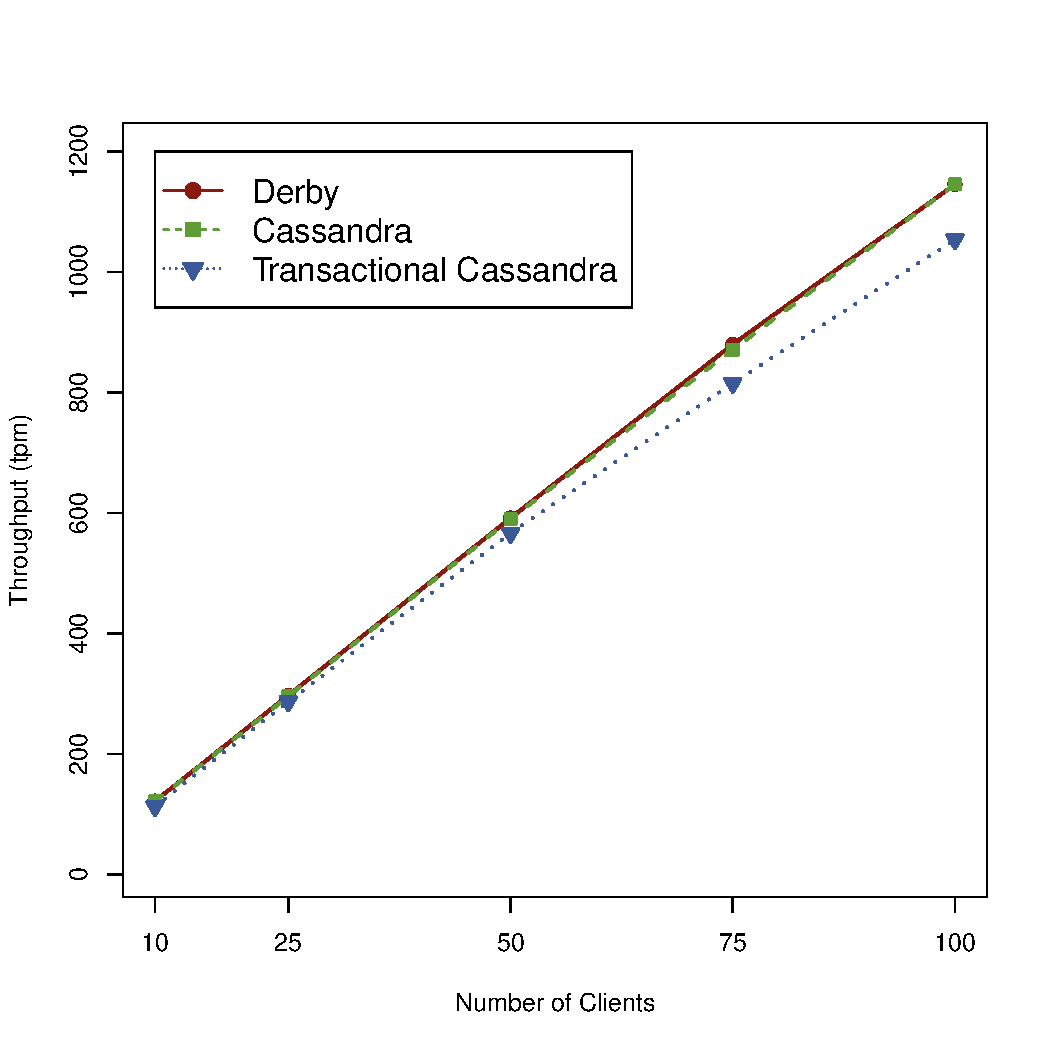
\includegraphics[width=0.7\textwidth]{images/tpcw_tpm.pdf}}\end{center}
  \begin{center}\subfigure[Latency]{\label{fig:lat10}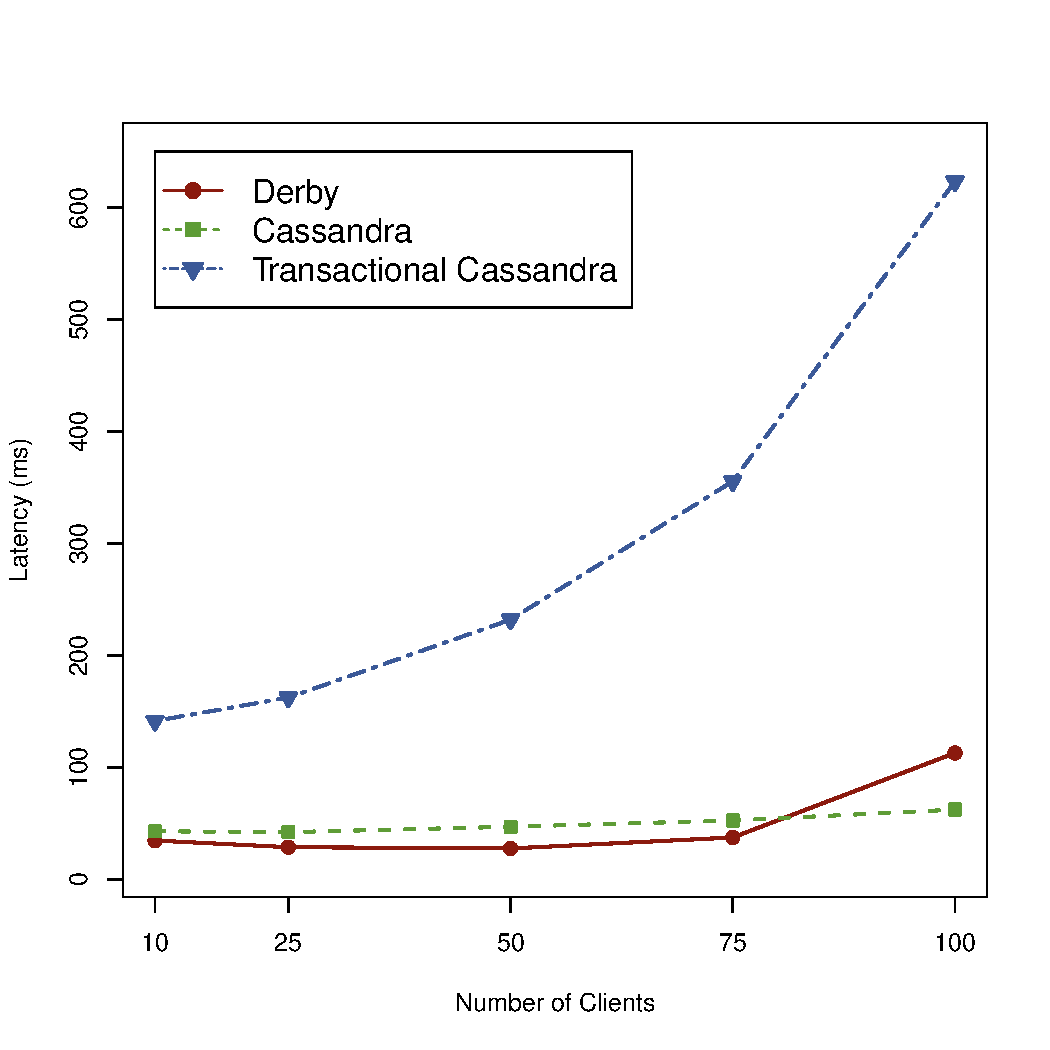
\includegraphics[width=0.7\textwidth]{images/tpcw_lat.pdf}}\end{center}
  \label{fig:tpcw10}
  \caption{Results of running TPC-W with different number of clients}
\end{figure}
 

\section{Yahoo! Cloud Serving Benchmark}

\ac{ycsb} is a framework presented by Yahoo!\footnote{\url{www.yahoo.com}} with the goal of facilitating performance comparisons of the new generation of cloud data serving systems. It focuses on \emph{serving} systems, which are systems that provide online read/write access to data such as Cassandra, as opposed to batch or analytical systems such as Hadoop~\cite{Cooper:2010:BCS:1807128.1807152}.

The workloads in the core package of \ac{ycsb} are a variation of the same application type. The application has one table of records each with \textbf{F} fields and identified by a primary key which is a string like ``user12345''. Each field is named \emph{field0}, \emph{field1}, and so on and has a random string of ASCII characters of length \textbf{L} as value. The operations against the data store are randomly chosen to be one of the following~\cite{Cooper:2010:BCS:1807128.1807152}:

\begin{description}
	\item[Insert] Insert a new record
	\item[Update] Update a record by replacing the value of multiple fields
	\item[Read] Read a record, either one randomly chosen field or all fields
	\item[Scan] Scan records in order, starting at a randomly chosen record key. The number of records to scan is randomly chosen from a configurable distribution (Uniform, Zipfian, Latest or Multinomial)
\end{description}

\ac{ycsb} also provides a tool called \ac{ycsb} Client to execute the benchmark, this tool has 5 workloads with different configurations. We introduced a new operation called multiupdate that performs updates on multiple rows, and to accommodate it we also created our own workload with 95\% reads, of which 80\% are actual read operations and 15\% are scans, and 5\% multiupdates.

For this test we used one machine running Cassandra for both the normal and transactional setting alongside with one zookeeper node for the latter. The results are shown for the scan operation are shown in figure \ref{fig:ycsb_scan}, for the read operation in figure \ref{fig:ycsb_read} and for the multiupdate in figure \ref{fig:ycsb_update}.

\begin{figure}[!ht]
  \subfigure[Scan]{\label{fig:ycsb_scan}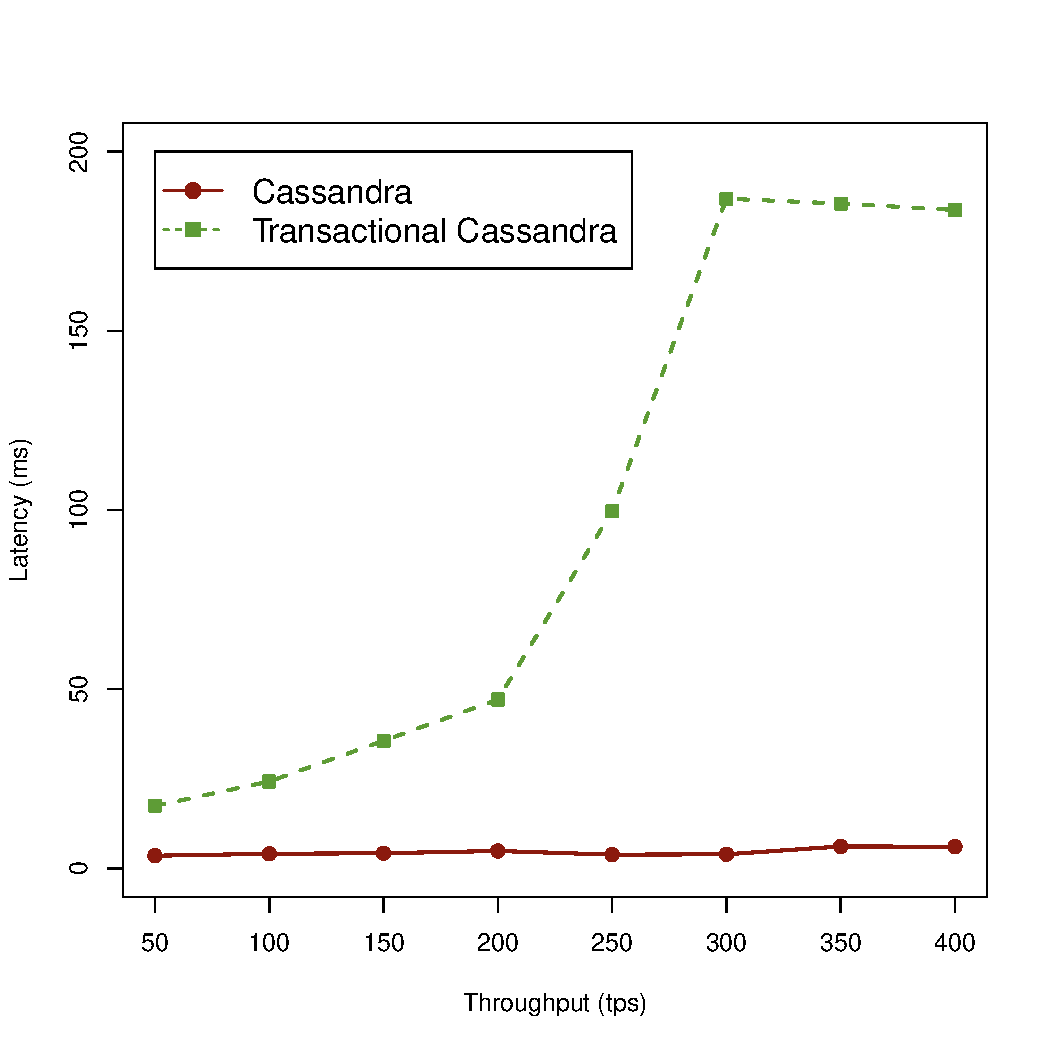
\includegraphics[width=0.5\textwidth]{images/ycsb_scan.pdf}}
  \subfigure[Read]{\label{fig:ycsb_read}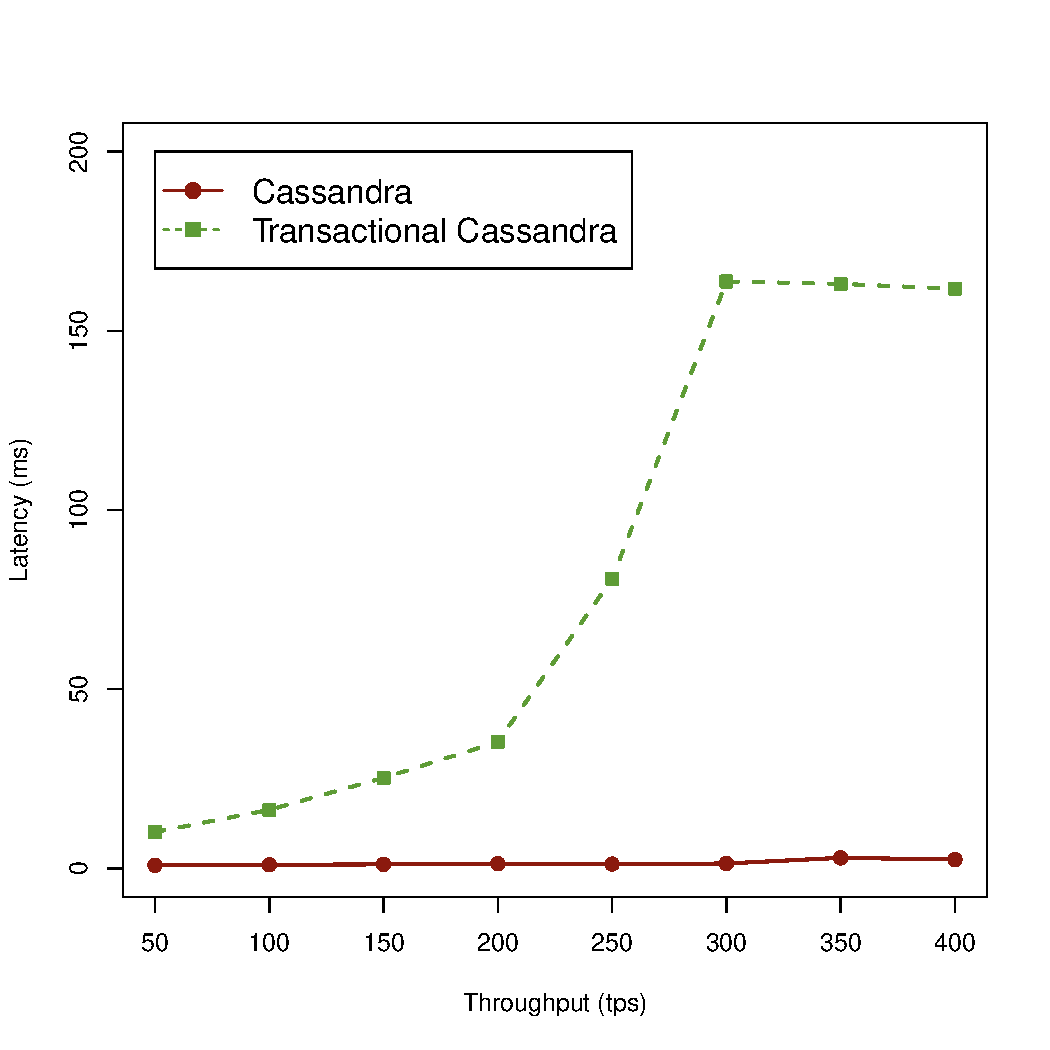
\includegraphics[width=0.5\textwidth]{images/ycsb_read.pdf}}
  \begin{center}\subfigure[Multiupdate]{\label{fig:ycsb_update}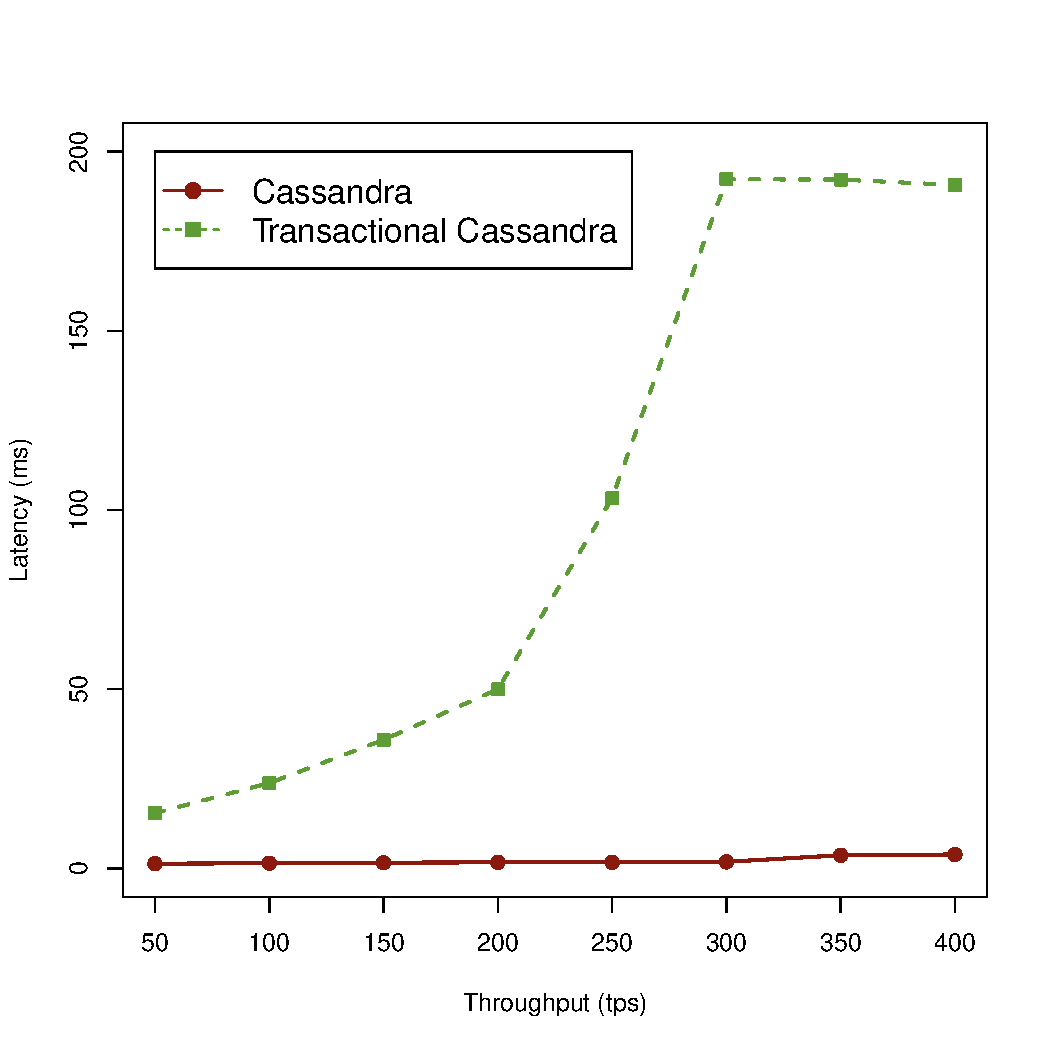
\includegraphics[width=0.5\textwidth]{images/ycsb_update.pdf}}\end{center}
  \label{fig:ycsb}
  \caption{Results of running YCSB with different expected throughput}
\end{figure}


\section{Scaling out}

So that we could better understand how the number of nodes in the cluster affected the system we tested its performance with 100 clients and 1000 items with the number of Cassandra nodes ranging from 1 to 5.  



   	   \mbox{}	
	%	\newpage
		\thispagestyle{plain}
		\mbox{}
   \chapter{Conclusions}
   	\label{sec:conclusion}
The lack of a standard querying \ac{api} and the relaxation in consistency alongside with the provided high availability, scalability and increased performance in certain use cases, makes \acp{vlsd} a thriving field of study and interest amongst the distributed systems community. However, all this properties also make it hard to migrate code from existing relational databases both because of the different interfaces and the lack of transactional guarantees so important in many scenarios.

With this work, we showed that it is possible to integrate a \ac{vlsd} with a \ac{rdbms} to the extent of providing an \ac{sql} interface for the former. In this context, the problems of such integration are described and a mapping of operations are proposed between DerbyDB and Cassandra.

In order to provide the transactional (ACID) guarantees, we propose a distributed transactions library based on a \ac{wal} mechanism and taking advantage of some of the guarantees of the actual \ac{vlsd}, in this case Cassandra. This library and how it can be integrated with the rest of the system is fully explained.

The tests performed show that ...  

Our system is modular and can be divided into four main parts:
\begin{description}
	\item[Applications (clients)] There can be multiple clients connect to the system
	\item[Core] Composed by the query engine and our abstraction layer, which contains the transactional system
	\item[Storage] This can be a cluster of multiple machines
	\item[Transactional Metadata] The metadata of the locking mechanism is stored in a Zookeeper cluster that can also be composed multiple machines
\end{description}

This modular approach combined with the provided functionality and new ideas makes this work a viable way to integrate legacy \ac{sql} code with a \ac{vlsd}. 

\section{Future Work}
The presented system solves the problems of providing an \ac{sql} interface and transactional functionality over a \ac{vlsd}. It has, however, certain limitations and some areas that can be further explored.

The main limitation of the system is that it does not provide snapshot isolation, this property comes directly from the fact that Cassandra does not allow multiple versions of a column.

This system is built specifically for the case of Derby and Cassandra and the transactional system is specially linked with Cassandra. An area to be explored would be building such a system for other \acp{vlsd} and if possible build a generic transactional system for most, if not all, \acp{vlsd}. 
   	\newpage
   	\thispagestyle{plain}
   	\mbox{}

%	\bibliographystyle{plain}
	\bibliographystyle{abbrv}
	\addcontentsline{toc}{chapter}{Bibliography}
	\bibliography{references}
	
	\appendix
		%\chapter{Additional Results}
		%	\section{MySQL Replication}

\subsection{Master and Multiples Slaves}

\begin{figure}[h!]
\centering    
\includegraphics[width=1\textwidth]{images/mms_semproxy/tt0_new/histo.pdf}
\caption{Replication delay values for Master and Multiple Slaves topology (no think-time)}
\end{figure}

\begin{figure}[h!]
\centering    
\includegraphics[width=1\textwidth]{images/mms_semproxy/tt03/histo.pdf}
\caption{Replication delay values for Master and Multiple Slaves topology (one-third of think-time)}
\end{figure}

\clearpage

\subsection{Chain}

\begin{figure}[h!]
\centering    
\includegraphics[width=1\textwidth]{images/chain/tt0_new/histo.pdf}
\caption{Replication delay values for Chain topology (no think-time)}
\end{figure}

\begin{figure}[h!]
\centering    
\includegraphics[width=1\textwidth]{images/chain/tt03/histo.pdf}
\caption{Replication delay values for Chain topology (one-third of think-time)}
\end{figure}

\clearpage

\section{Proxy Spread Plugins - Active Replication}

\subsection{FIFO Messages}

\begin{figure}[h!]
\centering    
\includegraphics[width=1\textwidth]{images/mms_comproxy_fifo/tt03/histo.pdf}
\caption{Replication delay values for active replication with Proxy Spread plugins with FIFO messages (one-third of think-time)}
\end{figure}

\clearpage


\subsubsection{Varying number of replicas}

\begin{figure}[h!]
\centering    
\includegraphics[width=1\textwidth]{images/mms_comproxy_fifo_varrepl/tt03_2repl/histo.pdf}
\caption{Replication delay values for active replication with Proxy Spread plugins with FIFO messages (one-third of think-time, two replicas)}
\end{figure}

\begin{figure}[h!]
\centering 
\includegraphics[width=1\textwidth]{images/mms_comproxy_fifo_varrepl/tt03_4repl/histo.pdf}
\caption{Replication delay values for active replication with Proxy Spread plugins with FIFO messages (one-third of think-time, four replicas)}
\end{figure}

\clearpage

\subsection{AGREED Messages}

\begin{figure}[h!]
\centering    
\includegraphics[width=1\textwidth]{images/mms_comproxy_agreed/tt03/histo.pdf}
\caption{Replication delay values for active replication with Proxy Spread plugins with AGREED messages (one-third of think-time)}
\end{figure}

\clearpage

\subsubsection{Varying number of replicas}

\begin{figure}[h!]
\centering    
\includegraphics[width=1\textwidth]{images/mms_comproxy_agreed_varrepl/tt03_2repl/histo.pdf}
\caption{Replication delay values for active replication with Proxy Spread plugins with AGREED messages (one-third of think-time, two replicas)}
\end{figure}

\begin{figure}[h!]
\centering    
\includegraphics[width=1\textwidth]{images/mms_comproxy_agreed_varrepl/tt03_4repl/histo.pdf}
\caption{Replication delay values for active replication with Proxy Spread plugins with AGREED messages (one-third of think-time, four replicas)}
\end{figure}
		%	
		%\chapter{Code and Scripts}
		%	\section{Lua Script to use on Proxy Spread Master Plugin}

\verb+ mysql-proxy --plugins=proxyspread_master --proxyspread-lua-script=spreadrepl.lua +\verb

\vspace{10mm}

\Large \textbf{spreadrepl.lua}\\
\small

\begin{lstlisting}
function read_query(packet)

	query = string.sub(packet, 2)
	
	--print("Seen the query: " .. query)	

	spread_send_msg(query)

end
\end{lstlisting}

\end{document}